%UNIT 14: NONLINEAR SYTEMS
%%%%%%%%%%%%%%%%%%%%%%%%%%%
%%%% Put the following at the top of each .tex file  %
\pagestyle{fancy}
\renewcommand{\theUnit}{14}
\ifthenelse{\isundefined{\UnitPageNumbers}}{}{\setcounter{page}{1}}
\rhead{Unit \theUnit: Nonlinear Systems}
\lhead{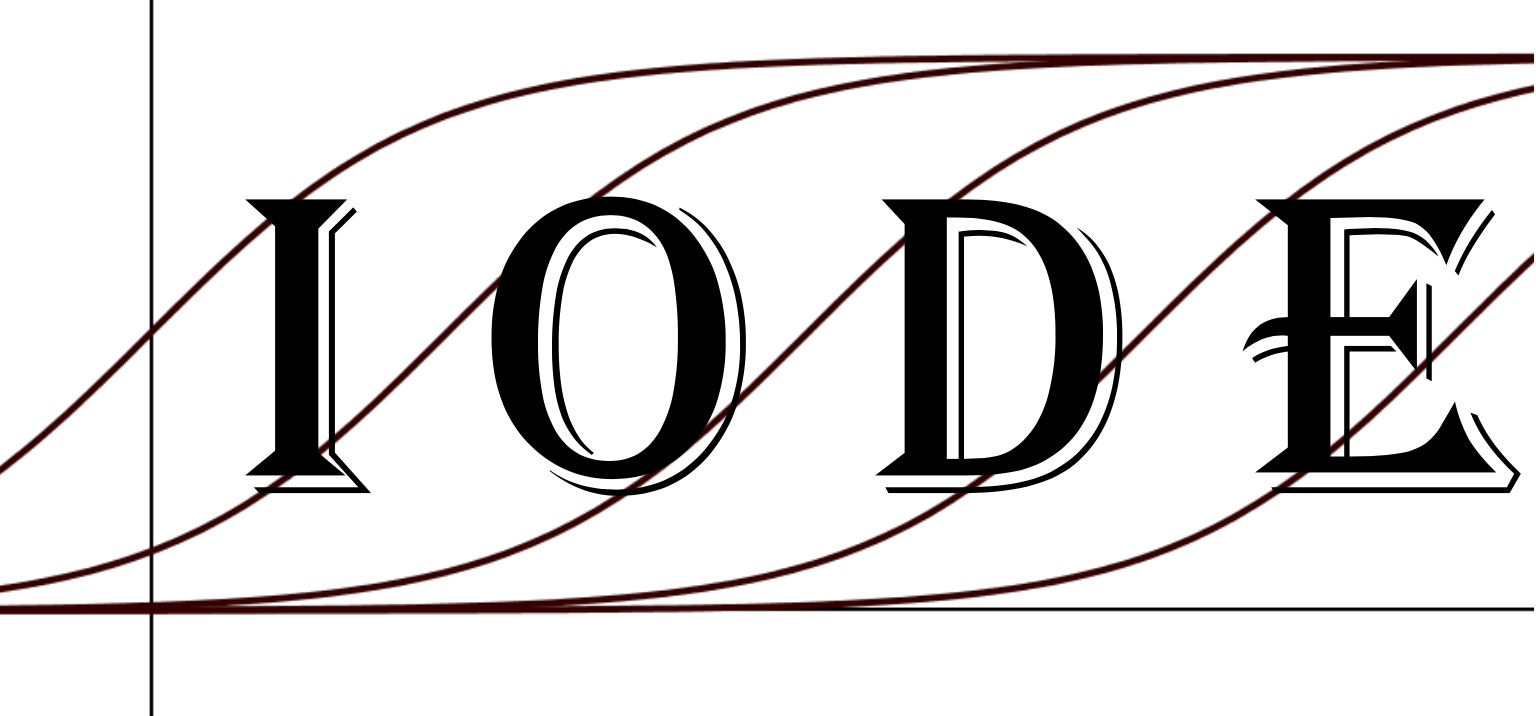
\includegraphics[width=1.25cm]{IODE-logo.png}}
\rfoot{\mypage}
\lfoot{}
\cfoot{}
\fancypagestyle{firstfooter}{\footskip = 50pt}
\renewcommand{\footrulewidth}{.4pt}
%%%%%%%%%%%%%%%%%%%%%%%%%%%
\vspace*{-20pt} \thispagestyle{firstfooter}
\pagebegin{In the Swing of Things}

A pendulum is attached to a wall in such a way that it is free to rotate around in a complete circle. Without provocation, Debra takes a baseball bat and hits it, giving it an initial velocity and setting it in motion. 
\begin{center}
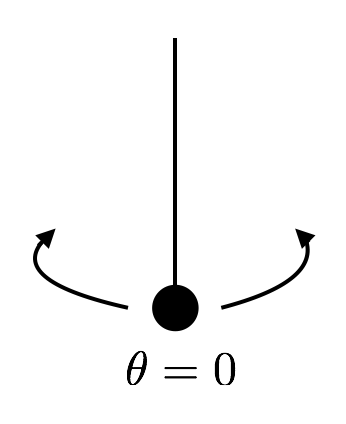
\includegraphics[width=1.5in]{14/14Pendulum1.png}
\end{center}
\begin{enumerate}
\item If we call $\theta$ the angular position of the pendulum (where $\theta = 0$ corresponds to when the pendulum is hanging straight down) and we call the velocity of the pendulum $v$, what would angular position versus velocity graphs look like for a variety of different initial velocities due to Debra's hit? Provide a brief description of the motion of the pendulum for your graphs. \label{14problem1}

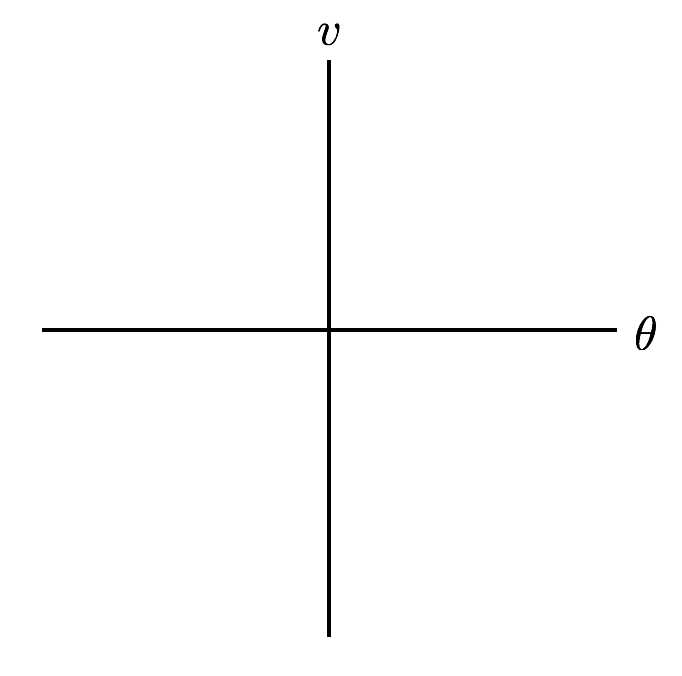
\includegraphics[width=3in]{14/14vtheta.png}
\item How many equilibrium solutions are there, where are they, and how would you classify them? \label{14problem2} \vfill
\end{enumerate}
\clearpage

Applying Newton's 2nd Law of motion (where $\theta = 0$ corresponds to the downward vertical position and counterclockwise corresponds to positive angles $\theta$) yields the differential equation
\[
\frac{d^2\theta}{dt^2}+\frac{b}{m}\frac{d\theta}{dt}+\frac{g}{l}\sin(\theta)=0
\]
where $b$ is the coefficient of damping, $m$ is the mass of the pendulum, $g$ is the gravity constant, and $l$ is the length of the pendulum (See homework problem \ref{14HWproblem5} for a derivation of this equation). Estimating the parameter values for the pendulum that Debra hits and changing this second order differential equation to a system of differential equations yields
\begin{align*}
\frac{d\theta}{dt} &=v \\
\frac{dv}{dt} &=-0.2v-\sin(\theta)
\end{align*}

\begin{enumerate}[resume]

\item How many equilibrium solutions does this system of differential equations have, where are they, and based on the context what types of equilibrium solutions would you expect them to be?  How does this connect with your answer to \ref{14problem2}? \label{14problem3} \vfill

\item You might recall that if $\theta$ is small, $\sin(\theta) \approx \theta$. Explain why this is true and then use this fact to approximate the above system with a linear system and classify the equilibrium solution at the origin. \label{14problem4} \vfill

\item Classify the equilibrium point at $\theta=\pi$. \label{14problem5} \vfill

\item Use the GeoGebra applet, \href{https://ggbm.at/SpfDSc5Q}{\underline{https://ggbm.at/SpfDSc5Q}}, to approximate the range of initial velocities with zero initial displacement that will result in the pendulum making exactly one complete rotation before eventually coming to rest. \label{14problem6}

\vspace{-.4in}\hspace{-.6in}
\includegraphics[width=.5in]{14/14PendulumQR.png}
\vfill
\end{enumerate}
\clearpage

%%%%%%%%%%%%%%%
\pagebegin{Linearization and Linear Stability Analysis}

In the next several questions we will develop tools to analyze equilibria of nonlinear systems.  To do this, we will first build our intuition by studying first order nonlinear equations.  

\begin{enumerate}[resume]
\item Recall from Calculus that the linearization, $L(h)$, of a function around a point of interest, $x^*$, is given by $L(h) \equiv f(x^*) + hf'(x^*)$. The key feature of the linearization is that, when $x \approx x^*$, that is, $x=x^*+h$ for $h \approx 0$, then $f(x) \approx L(h)$. \label{14problem7}

\begin{tabular}{|p{2.5in}|p{3in}|}
\hline
Find the linearization of $f(x)=1-x^2$ around $x^*=1$. \vspace{1.25in} &  \\ \hline
If $x \approx 1$, $x$ can be written as $x=1+h$ where $h \approx 0$. Suppose $x$ follows the differential equation $\frac{dx}{dt}=1-x^2$. Use the linearization above to write down a linear differential equation for $\frac{dh}{dt}$. \vspace{1.25in} &  \\ \hline
According to the above differential equation, what is the long term behavior of $h$? &  \\ \hline
If $x(0) \approx 1$, what does the long term behavior of $h$ tell you about the long term behavior of $x$? &  \\ \hline
\end{tabular}

\item \label{14problem8}
\begin{enumerate}
\item Consider again $\displaystyle\frac{dx}{dt}=1-x^2$, but this time with $x(0) \approx -1$. Find a new linearization and use it to make a long term prediction about $x$. \label{14problem8parta} \vfill

\clearpage

\item Why was it necessary to construct a \textbf{new} linearization to study $x(0) \approx -1$? \label{14problerm8partb} \vfill

\item Using linearization to determine the stability of a critical point is called ``linear stability analysis.'' Use a phase line to corroborate your linear stability analysis. \label{14problem8partc} \vfill

\item For an arbitrary system, $\displaystyle\frac{dx}{dt}=f(x)$ with an equilibrium point at $x=x^*$, describe how you can use linear stability analysis to determine the stability of the equilibrium point. \label{14problem8partd} \vfill
\end{enumerate}

\item Consider the following system: \label{14problem9}
\begin{align*}
\frac{dx}{dt} &= 1-x^2 \\
\frac{dy}{dt} &= -3x -3y
\end{align*}
\begin{enumerate}
\item Algebraically find the equilibrium solutions. \label{14problem9parta} \vfill
\item Tanesha used the GeoGebra Vector field applet, \href{https://ggbm.at/kkNXUVds}{\underline{https://ggbm.at/kkNXUVds}}, to plot the vector field associated with the differential equation.  Based on this vector field, how would you classify the equilibria? \label{14problem9partb}

\vspace{-.25in}\hspace{-.75in}
\includegraphics[width=.5in]{14/14VectorFieldQR.png}
\vfill
\end{enumerate}
\end{enumerate}

\clearpage

We can also perform linear stability analysis on a system of two or more variables, such as the one in the previous problem. Consider a function $f(x,y)$, then Taylor's theorem states that, if $(x,y) \approx (x^*,y^*)$, that is, if $(x,y) = (x^*+h_1, y^*+h_2)$ where $h_1 \approx 0$ and $h_2 \approx 0$, then
\[
f(x,y) \approx L(h_1,h_2) = f(x^*,y^*) + h_1f_x(x^*,y^*) + h_2f_y(x^*,y^*)
\]
where $f_x$ and $f_y$ are the partial derivatives of $f$ with respect to $x$ and $y$, respectively. \\

$L(h_1,h_2)$ is called the linearization of $f(x,y)$ around $(x^*,y^*)$.

\begin{enumerate}[resume]
\item Consider the system of differential equations:
\begin{align*}
\frac{dx}{dt} &= 1-x^2 \\
\frac{dy}{dt} &= -3x -3y
\end{align*}
Let's first study the equilibrium at (1,-1). \label{14problem10}

\begin{tabular}{|p{2.5in}|p{3in}|}
\hline
If the system had $x(0) \approx 1$ and $y(0) \approx -1$, we could write $x=1+h_1$ and $y=-1+h_2$, with $h_1 \approx 0$ and $h_2 \approx 0$. Use the linearization of the original system of equations around $(1,-1)$ to write down a system of differential equations for $h_1$ and $h_2$ \vspace{1.5in} &  \\ \hline
What are the long term behaviors of $h_1$ and $h_2$? \vfill &  \\ \hline
What can you conclude about the long term behaviors of $x$ and $y$? \vfill &  \\ \hline
Classify the equilibrium point $(1,-1)$, according to your linear stability analysis. \vfill &  \\ \hline
\end{tabular}

\clearpage

\item \label{14problem11}
\begin{enumerate}
\item Consider again
\begin{align*}
\frac{dx}{dt} &= 1-x^2 \\
\frac{dy}{dt} &= -3x -3y
\end{align*}
Use linear stability analysis to classify the equilibrium point at $(-1,1)$. \label{14problem11parta} \vfill
\item Combine your results from question \ref{14problem10} and \ref{14problem11parta}, to sketch a possible phase plane for the system of differential equations. Does an analysis of the system using nullclines corroborate your linear stability analysis? \label{14problem11partb} \vfill
\end{enumerate}

\clearpage

\item For a system of differential equations
\begin{align*}
\frac{dx}{dt} &= f(x,y) \\
\frac{dy}{dt} &= g(x,y)
\end{align*}
with an equilibrium point at $(x^*,y^*)$, the matrix
\[
J =
\begin{bmatrix}
f_x(x^*,y^*) & f_y(x^*,y^*) \\
g_x(x^*,y^*) & g_y(x^*,y^*)
\end{bmatrix}
\]
is called the \textbf{Jacobian matrix}. Explain how you can use the Jacobian matrix to determine the behavior of a the system of differential equations near $(x^*,y^*)$. \label{14problem12} \vfill

\item Use linear stability analysis to classify the critical points you found in the pendulum system. \label{14problem13}
\begin{align*}
\frac{d\theta}{dt} &=v \\
\frac{dv}{dt} &= -0.2v - \sin(\theta)
\end{align*}
\vfill

\end{enumerate}

\clearpage

\pagebegin{Homework Set 14}

\begin{enumerate}
\item \underline{Bees and Flowers II}. In an earlier problem, we studied systems of rate of change equations designed to inform us about the future populations for two species that are either competitive (that is both species are harmed by interaction) or cooperative (that is both species benefit from interaction). \label{14HWproblem1}

\begin{center}
\begin{tabular}{cc}
	 (A)	&	(B)	\\
$\displaystyle \begin{aligned} \frac{dx}{dt} &= -5x+2xy\\ \frac{dy}{dt} &= -4y+3xy \end{aligned}$ &$\displaystyle \begin{aligned} \frac{dx}{dt} &= 3x(1-\frac{x}{3})-\frac{1}{10}xy\\ \frac{dy}{dt} &= 2y(1-\frac{y}{10})-\frac{1}{5}xy \end{aligned}$ 
\end{tabular}
\end{center}

\begin{enumerate}
\item Explain why the second system of rate of change equations describes a situation where the two species are competitive. \label{14HWproblem1parta}
\item Verify that the equilibrium solutions for system (B) are (0,0), (3, 0), (0, 10), and $(\frac{20}{9},\frac{70}{9})$. \label{14HWproblem1partb}
\item Determine the linearized system of differential equations about each equilibrium solution and use the information you gain about the solutions near each of these equilibrium solutions to sketch the phase portrait. \label{14HWproblem1partc}
\end{enumerate}

\item Without using technology, use the tools of linearization and nullclines to sketch the phase portrait for the nonlinear system: \label{14HWproblem2}
\begin{align*}
\frac{dx}{dt} &=\cos(y) \\
\frac{dy}{dt} &=y-x
\end{align*}
Be as accurate as possible and show all supporting work.

\item When the John Hancock Building in Boston, MA was first built it tended to sway back and forth so much so that people in the top floors experienced motion sickness. Similar to the spring mass system, we can model the back and forth motion of the building by adding a gravity term to the spring mass model.
 
The following system of rate of change equations is a model for helping us make predictions about the motion of a skyscraper swaying in the wind. In this simplified system of rate of change equations, $x$ is the amount of displacement of the building from the vertical position at any time $t$ and $y$ is the horizontal velocity of the building at any time $t$. Use what you know about linear stability analysis to analyze the behavior of the systems at the critical points and compare to your earlier work. (You might want to use a GeoGebra vector field applet, \href{https://ggbm.at/kkNXUVds}{\underline{https://ggbm.at/kkNXUVds}}, to help understand it first). \label{14HWproblem3}

\vspace{-.5in}\hspace{-.6in}
\includegraphics[width=.5in]{14/14VectorFieldQR.png}
\begin{align*}
\frac{dx}{dt} &=y \\
\frac{dy}{dt} &=-x-y+x^3
\end{align*}

\clearpage

\item Consider the phase plane below for the damped pendulum: \label{14HWproblem4}
\begin{center}
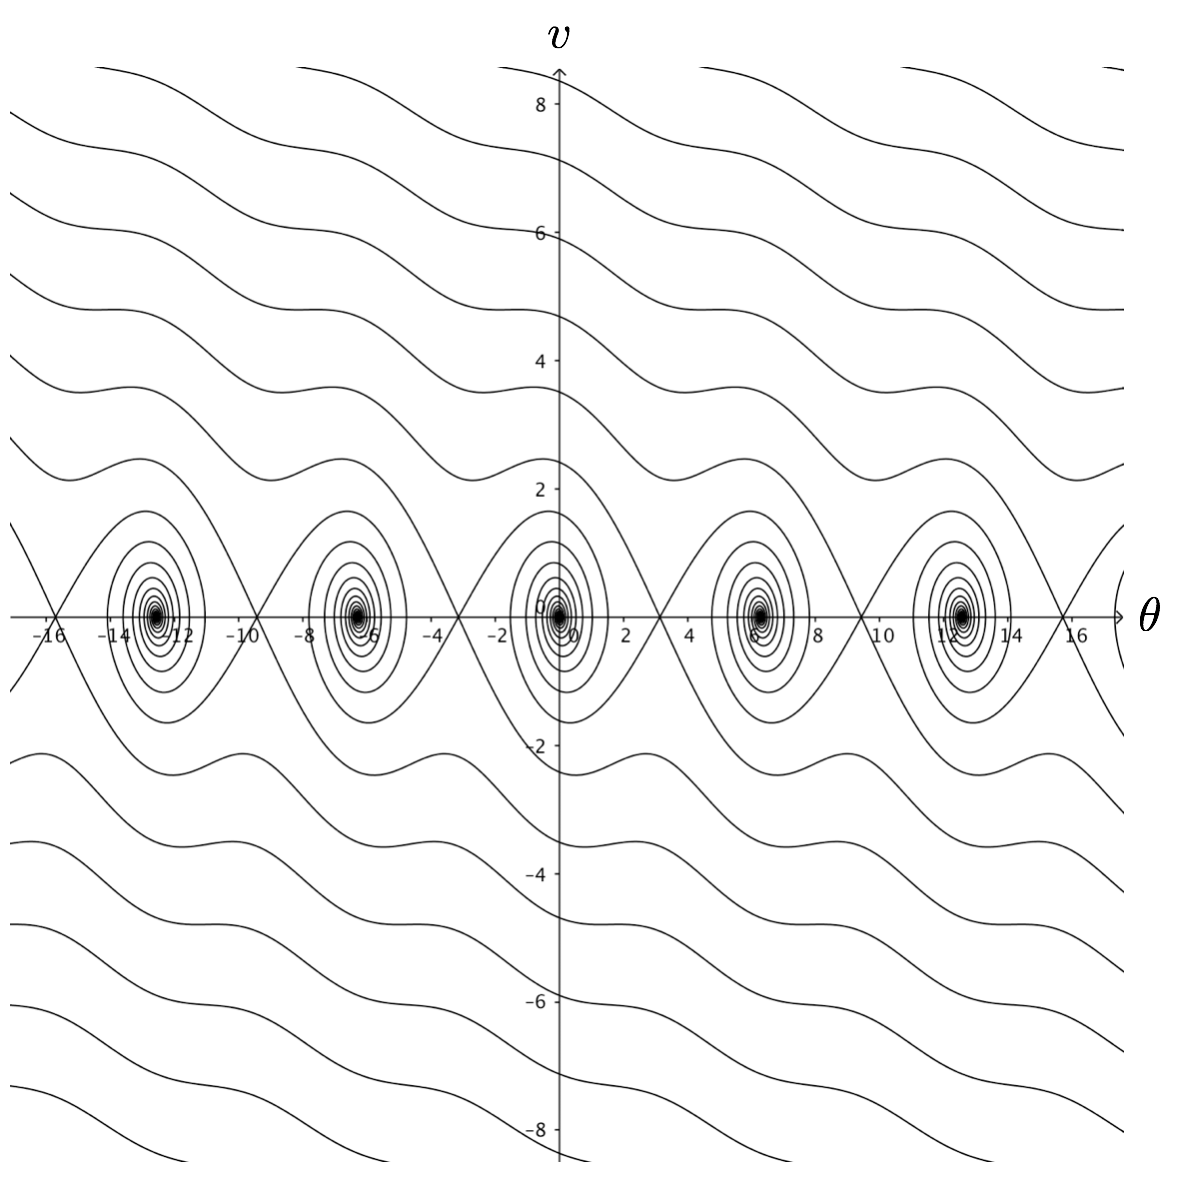
\includegraphics[width=5in]{14/14HWphaseplane.png}
\end{center}
\begin{enumerate}
\item Shade in the region(s) corresponding to initial conditions that will make one full revolution before coming to a stop. \label{14HWproblem4parta}
\item Use a different shading to show the region(s) corresponding to initial conditions that will make two full revolutions before coming to a stop. \label{14HWproblem4partb}
\end{enumerate}

\clearpage

\item Consider the diagram below for the pendulum: \label{14HWproblem5}
\begin{center}
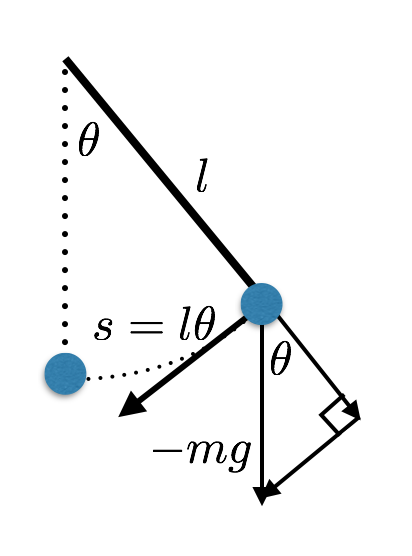
\includegraphics[width=2in]{14/14Pendulum2.png}
\end{center}
\begin{enumerate}
\item The force, due to gravity, on the bob of the pendulum is given by $-mg$. Explain why the proportion of that gravitational force, in the direction tangent to the path of the pendulum's bob, is given by $F=-mg\sin(\theta)$. \label{14HWproblem5parta}
\item In the diagram above, explain why the length of the dotted arc is given by $s=l\theta$, when $\theta$ is measured in radians. \label{14HWproblem5partb}
\item The frictional force (due to friction at the fixed point of the pendulum, or due to air resistance, or a combination of these two) opposes the motion of the pendulum. Carefully explain why this force can be represented as $F=-b\displaystyle\frac{ds}{dt} = - bl\displaystyle\frac{d\theta}{dt}$. \label{14HWproblem5partc}
\item Newton's law states that force is given by mass times acceleration. If $m$ is the mass of the pendulum bob, explain why $F=m\displaystyle\frac{d^2s}{dt^2} = ml\displaystyle\frac{d^2\theta}{dt^2}$. \label{14HWproblem5partd}
\item Explain how the previous parts of this question can be combined to arrive at a differential equation: \label{14HWproblem5parte}
\[
ml\frac{d^2\theta}{dt^2} = -bl\frac{d\theta}{dt} - mg\sin(\theta)
\]
\item By defining $v=\displaystyle\frac{d\theta}{dt}$, develop a pair of first order differential equations for the $(\theta,v)$ system. \label{14HWproblem5partf}
\end{enumerate}

\end{enumerate}




